\documentclass[letterpaper,12pt]{article}
\usepackage{mathtools}
\DeclarePairedDelimiter\abs{\lvert}{\rvert}     %serve per mettere il modulo 
\usepackage{booktabs}
\usepackage{bm}
\usepackage{textcomp}
\usepackage{colortbl}
\usepackage{tabularx}
\usepackage{textcomp}
\usepackage{siunitx}
\usepackage{booktabs}
\usepackage{enumitem}
\usepackage{xcolor}
\usepackage{fancyhdr}
\usepackage{caption}
\usepackage{changepage}
\usepackage{amsmath} 
\usepackage{subcaption}
\usepackage{graphicx}
\usepackage[table]{xcolor} 
\usepackage[margin=1in,letterpaper]{geometry} % decreases margins
\usepackage{cite} % takes care of citations
\usepackage[hidelinks]{hyperref} % adds hyper links inside the generated pdf file
\usepackage{siunitx} % provides the \SI{}{} command for proper typesetting of units
% Define the colors
\definecolor{linkcolor}{RGB}{0, 102, 204}
\definecolor{citecolor}{RGB}{34, 139, 34}
\definecolor{urlcolor}{RGB}{255, 69, 0}

% Setup hyperref
\hypersetup{
    colorlinks=false, % colored links
    linkcolor=linkcolor, % color for internal links
    citecolor=citecolor, % color for citations
    urlcolor=urlcolor, % color for URLs
}
\fancypagestyle{logoheader}{
    \fancyhf{}
    \fancyhead[L]{
\includegraphics[width = 3cm]{infn-art-science-universita-degli-studi-di-milano-bicocca-maintainer-universita-studi-milano-bicocca.png}}
    \renewcommand{\headrulewidth}{0pt}
    }
\usepackage{blindtext}
\graphicspath{{immagini/}}
%Required for inserting images
%++++++++++++++++++++++++++++++++++++++++
%Margini 



\begin{document}

\title{{\small Università degli studi Milano-Bicocca  Dipartimento di Fisica - Laboratorio II }\\
	Esperienza Ottica - Microonde}
\author{F. Ballo, S. Franceschina, S. Dolci - Gruppo T1 39}
\date{\today}
\maketitle
\thispagestyle{logoheader}


\begin{abstract}
	Nella seguente relazione vengono presentati i risultati ottenuti dalla quinta esperienza del corso di 
    Laboratorio II riguardante l'analisi di fenomeni ottici che rientrano nel campo della spettrometria. L'obiettivo di questa esperienza è quello di capire come
    identificare un elemento una volta noto il suo spettro di emissione.
	\begin{adjustwidth}{-1cm}{-1cm}
	\end{adjustwidth}
\end{abstract}
\tableofcontents
\newpage

\section{Configurazione setup esperienza}
Per le misure di questa esperienza abbiamo utilizzato:

\begin{itemize}
    \item Uno spettrometro PASCO scientific Modello SP-9416, \href{https://cdn.pasco.com/product_document/Student-Spectrometer-Manual-SP-9268A.pdf}{manuale qui.}
    \item Lampade ad incadescenza Hg, Na e gas ignoti.
    \item Prisma di vetro flint.
    \item Reticoli di diffrazione 300/600/1200 (linee/mm).
\end{itemize}
Prima della presa di misure abbiamo verificato la calibrazione degli strumenti regolando la messa a fuoco e 
l'apertura della fenditura usando come sorgente test una lampada al Na.
    
\section{Prisma}
La prima parte dell'esperienza ha come obiettivo la caratterizzazione dell'indice di rifrazione del prisma, 
grazie al quale è poi possibile avanzare delle ipotesi sulla natura di sorgenti gas ignoti. Come configurazione, sia per
la sezione di caratterizzazione del prisma che per quella di identificazione del gas ignoto, abbiamo utilizzato il setup
riportato in figura \ref{fig:SetupPrisma}.
\begin{figure}[h!]
	\centering
	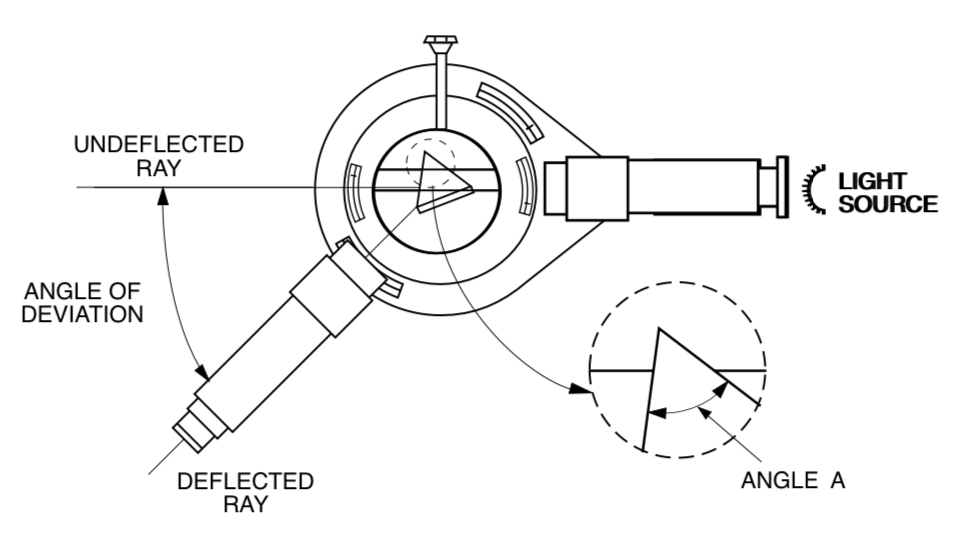
\includegraphics[width = 0.5\textwidth]{SetupIniziale.jpeg}
	\caption{Configurazione spettrometro con prima per misure d'angolo}
	\label{fig:SetupPrisma}
\end{figure}

\begin{figure}[h!]
	\centering
	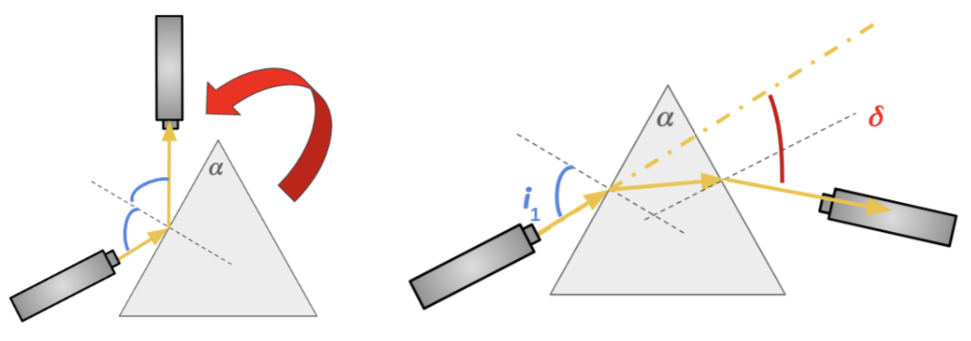
\includegraphics[width = 0.5\textwidth]{Prisma.jpeg}
	\caption{Configurazione prisma}
	\label{fig:Prisma}
\end{figure}


\subsection{Caratterizzazione del prisma}
Dopo aver riprodotto la configurazione riportata in figura \ref{fig:SetupPrisma}, abbiamo utilizzato una lampada al 
mercurio come sorgente. Abbiamo misurato l'angolo di minima deviazione $\delta$ e da questo abbiamo calcolato l'indice 
di rifrazione del prisma per i vari colori utilizzando la relazione $\sin(\frac{\delta + \alpha}{2}) = n \sin(\frac{\delta}{2})$.
Una volta ottenuti gli indici di rifrazione al variare delle lunghezze d'onda tabulate abbiamo potuto interpolare 
la relazione \ref{eq:Cauchy} per ottenere i parametri $A$ e $B$.
\begin{equation}
    n(\lambda) = A + \frac{B}{\lambda^2}
    \label{eq:Cauchy}
\end{equation}

Riportiamo in figura \ref{fig:Cauchy_fit} il fit ottenuto e i parametri $A$ e $B$ ottenuti.
\begin{figure}[h!]
    \centering
    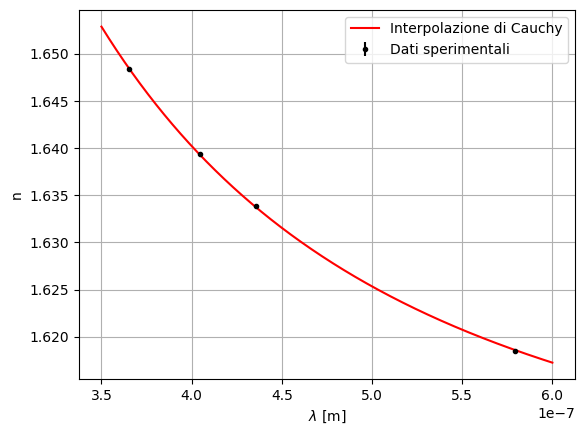
\includegraphics[width = 0.5\textwidth]{Cauchy_fit.png}
    \caption{Interpolazione secondo la relazione di Cauchy}
    \label{fig:Cauchy_fit}
\end{figure}

Abbiamo ottenuto i seguenti parametri:
\begin{itemize}
    \item $A = 1.599 \pm 0.0003$
    \item $B = (0.0061 \pm 0.0005) \mu$m
    \item $\tilde{\chi}^2 = 1.0$
\end{itemize}

\subsubsection{Considerazioni sugli errori}

\subsection{Identificazione del gas ignoto}

\section{Reticolo di diffrazione}

\subsection{Caratterizzazione del reticolo}

\subsection{Identificazione del gas ignoto}

\newpage
\section{Tabelle}

\end{document}